\section{Adiabatic Gradient Variations}
\label{alldelad}

\subsection{Adiabatic Gradient during Partial Dissociation}\label{deladdiss}

%The adiabatic gradient during dissociation or ionization is a function of temperature and the dissociation or ionization fraction $x$. The Saha equation (e.g., \citealt{kippenhahn90}) relates $x$ to the gas 


The total internal energy of a partially dissociated gas includes contributions from the individual internal energies of the molecules and atoms, as well as from the dissociation energy. The dissociation energy depends on the dissociation fraction $x$ (i.e., the fraction of molecules that have dissociated), which can be found from the Saha equation (see e.g., \citealt{kippenhahn90}, Chapter 14) as a function of temperature and density,

\begin{equation}
\label{eq:saha}
\frac{x^2}{1-x} \propto \frac{T^{3/2}}{\rho} e^{-\chi/k_B T},
\end{equation} 
where $\chi$=4.48 eV is the dissociation energy for molecular hydrogen \citep{blanksby03}.

The above also holds true for ionization, with the dissociation energy replaced by ionization energy $\chi=13.6$ eV for atomic hydrogen \citep{mandl89}. From the Saha equation one can find an expression for $\rho$ as a function of $T$ and $x$, then derive the adiabatic gradient directly from its definition (Equation \ref{eq:delad}), taking into account the fact that the mean molecular weight in the ideal gas law varies with $x$, hence the pressure will not only be a function of $T$ and $\rho$ but also of $x$ (see \citealt{kippenhahn90}, Chapter 14.3 for a detailed derivation). The final expression for the adiabatic gradient during ionization is 

\begin{equation}
\label{eq:deladioniz}
\delad=\frac{2+x (1-x) \Phi_H}{5+x(1-x)\Phi_H^2},
\end{equation}
with $\Phi_H \equiv \frac{5}{2}+\frac{\chi}{k_B T}$. The derivation of $\delad$ during dissociation is more involved mathematically (see, e.g., \citealt{vardya60}) and leads to a slightly more complicated final expression,

%One can derive a simple expression for the adiabatic gradient as a function of $x$ and $T$ from it's definition (equation \ref{eq:delad}), using the 

%The adiabatic gradient follows as (see \citealt{vardya60} for a detailed derivation)

\begin{equation}
\label{eq:deladdiss}
\delad=\frac{1+x+ \frac{x(1-x^2)}{2} \frac{\chi}{k_B T}}{5 x + \frac{7(1-x)}{2} + \frac{x(1-x^2)}{2} \Big(\frac{\chi}{k_B T}\Big)^2} \, .
\end{equation} 
Using Equation (\ref{eq:deladdiss}), we recover $\delad=2/7$ for $x=0$ (no ongoing dissociation hence hydrogen is purely molecular and diatomic) and $\delad=2/5$ for $x=1$ (hydrogen is fully dissociated into atoms and hence monatomic). Figure \ref{fig:deladdiss} shows the dependence of $\delad$ on the dissociation fraction, for $T=3000$ K, the temperature at which dissociation typically occurs \citep{langmuir12}. The adiabatic gradient drops substantially during partial dissociation, since part of the internal energy is used in dissociation rather than in increasing the temperature of the system.


\begin{figure}[h]
\centering
%\includegraphics[width=0.5\textwidth]{../../figs/ModelAtmospheres/RadSelfGravRealEOS/PaperFigs/delad_dissociation.pdf}
\includegraphics[width=0.5\textwidth]{figures/delad_dissociation.pdf}
%%\vspace{-0.5in}
\caption{Adiabatic gradient as a function of the hydrogen dissociation fraction $x$. The adiabatic gradient is $\delad=2/7$ for pure molecular hydrogen ($x=0$) and $\delad=2/5$ for fully atomic hydrogen ($x=1$), and drops to low values during partial dissociation.}
\label{fig:deladdiss}
\end{figure}


\subsection{Adiabatic Gradient during Conversion of Spin Isomers}
\label{deladspin}

The adiabatic gradient scales as $\delad \sim 1/c_{\rm V}$.
%  where $c_{\rm V} \sim c_{\rm V,t}+c_{\rm V,r}$.
% is the specific heat capacity at constant volume and $c_{\rm V, t}$ and $c_{\rm V,r}$ are the translational and rotational components, respectively.  
The translational component of the heat capacity, $c_{\rm V, t}=3\mathcal{R}/2$, is independent of temperature.  As $c_{\rm V,r}$ increases, $\delad$ declines. We can therefore understand how conversion between spin isomers affects $\delad$ by studying the dependence on temperature of $c_{\rm V, r}$ of the ortho-para mixture. 

The internal energy per unit mass and specific heat capacity associated with rotation for the individual isomers, for the equilibrium mixture, and for a fixed ortho-para ratio of 3:1 can be derived from their partition functions (see \App{EOStables} for details), and are plotted in Figure  \ref{fig:ucvr} (after \citealt{farkas35}, Figure 1). At low temperatures, parahydrogen is in the $j=0$ state and has no rotational energy, while orthohydrogen is in the $j=1$ state and has the energy of its first rotational level. Both para- and orthohydrogen, as well as their equilibrium mixture, behave like monatomic gases at low temperatures and thus have zero rotational heat capacity. This is consistent with $\delad=2/5$ at low temperatures as seen in Figure \ref{fig:deladmap}. As the temperature increases, the energetically higher-lying rotational states of para- and orthohydrogen are populated and the heat capacity of both spin isomers increases as a result. We note that the heat capacity of the equilibrium mixture is not a weighted average of the heat capacities of the individual components because it takes into account both the rotational energy uptake of para- and orthohydrogen, and also the shift in their equilibrium concentrations with temperature. This results in a peak in the heat capacity of the mixture around $\sim$$50$ K, as seen in the bottom plot of Figure \ref{fig:ucvr}. It follows that the adiabatic gradient has to reduce, reach a minimum, then increase as the temperature rises, as shown in Figure \ref{fig:deladmap}. In contrast, the heat capacity for the 3:1 ortho-para ratio mixture will be a weighted average between the individual ortho- and para- components, and will hence have intermediate values between the two, as displayed in Figure \ref{fig:ucvr}.

Figure \ref{fig:Lt_31}, bottom panel, shows that the atmospheric growth time may increase by a factor of $\sim$$3$ if a fixed 3:1 ortho-para ratio is assumed instead of thermal equilibrium between the hydrogen spin isomers.  This enhanced growth time  increases $M_{\rm crit}$. 

% As the temperature increases, the energetically higher-lying ($j=1$) ortho-hydrogen is formed, and the concomitant energy increase is seen as a peak in the heat capacity of the equilibrium mixture. 


%There are two significant maxima in the heat capacities of parahydrogen and of the mixture. At very low temperatures, the heat capacity of parahydrogen is zero because only the lowest accessible energy level $j=0$ is occupied and a temperature increase does not provide enough energy to populate the next higher level. When the temperature becomes sufficiently high to populate the second lowest level $j=2$, the heat capacity rapidly increases, passes through a maximum and starts to decrease when the second lowest level becomes saturated. 


%the adiabatic gradient is inversely proportional to the heat capacity, it 

%means that  the former has to first decrease from 2/5 as the temperature increases, reach a minimum around 50 K ($\delad \approx 0.25$ from Fig. \ref{fig:deladmap}), then gradually increase to 2/7 as for a diatomic gas. This behavior is illustrated in Figure \ref{fig:deladmap}.  



%The maxima in the ortho-para mixture appears when parahydrogen starts converting into orthohydrogen. The heat capacity of the equilibrium mixture is not a weighted average of the heat capacities of the individual components because it takes into account both the rotational energy uptake of para- and orthohydrogen, and also the shift in their equilibrium concentrations with temperature. At $T=0$, only parahydrogen is present in the equilibrium mixture; as the temperature is increased, the energetically higher-lying ($j=1$) ortho-hydrogen is formed, and the concomitant energy increase is seen as a peak in the heat capacity. As the adiabatic gradient is inversely proportional to the heat capacity, it means that  the former has to first decrease from 2/5 as the temperature increases, reach a minimum around 50 K ($\delad \approx 0.25$ from Fig. \ref{fig:deladmap}), then gradually increase to 2/7 as for a diatomic gas. This behavior is illustrated in Figure \ref{fig:deladmap}.  



\begin{figure}[h]
\centering
%\includegraphics[width=0.5\textwidth]{../../figs/ModelAtmospheres/RadSelfGravRealEOS/PaperFigs/ortho_para_energy.pdf}
\includegraphics[width=0.5\textwidth]{figures/ortho_para_energy.pdf}
%%\vspace{-0.5in}
\caption{Internal energy per unit mass and specific heat capacity associated with rotation for parahydrogen (dashed blue), orthohydrogen (dotted green), the equilibrium mixture (solid red) and a fixed 3:1 ortho-to-para ratio (dash-dotted light blue) as a function of temperature. After \citet{farkas35}, Figure 1.}
\label{fig:ucvr}
\end{figure}

\begin{figure}[h]
\centering
%\includegraphics[width=0.5\textwidth]{../../figs/ModelAtmospheres/RadSelfGravRealEOS/PaperFigs/Ltplot_31.pdf}
\includegraphics[width=0.5\textwidth]{figures/Ltplot_31.pdf}
%%\vspace{-0.5in}
\caption{Evolution of the luminosity and elapsed time during atmospheric growth around a $8 M_{\oplus}$ core at 100 AU, for a realistic EOS with hydrogen spin isomers in thermal equilibrium (solid line), and with a fixed ortho-to-para ratio 3:1 (dashed line). The assumption of a fixed ortho-to-para ratio increases the runaway accretion time $t_{\rm run}$ by a factor of $\sim$$3$ compared to the equilibrium mixture.}o
\label{fig:Lt_31}
\end{figure}


%with $\chi$ and $T$ the dissociation energy and temperature, respectively, equal to $\chi=4.48$ eV\citep{blanksby03} and $T\sim3000$ K \citep{langmuir12} for molecular hydrogen.

%Specifically, if we denote the internal energies of neutral hydrogen, protons and electrons as $U_{H}$, $U_+$ and $U_e$, respectively, then the total internal energy of the gas is given by:

%\begin{equation}
%U=U_H+U_+ + U_e + x \chi,
%\end{equation}
%
%\noindent where $x$ is the ionization fraction and $\chi$ is the ionization energy (equal to -13.6 eV for hydrogen). The ionization fraction can be determined from the Saha equation (see e.g., \citealt{kippenhahn90}).
%
%\begin{equation}
%\label{eq:saha}
%\frac{x^2}{1-x} \frac{\rho}{m_H}=\frac{(2 \pi m_e k_B T)^{3/2}}{h^3} e^{-\chi/k_B T},
%\end{equation}
%
%\noindent where $m_e$ is the mass of the electron and $h$ is Planck's constant. It can be seen from the Saha equation that the ionization fraction depends only on the gas temperature and density: $x=x(T, \rho)$. As such, all the thermodynamic quantities also depend only on the gas temperature and density, and hence on the equation of state. The adiabatic gradient is given by (see \citealt{kippenhahn90}, chapter 14 for a derivation):
%
%\begin{equation}
%\delad=\frac{2+x (1-x) \Phi_H}{5+x (1-x) \Phi_H^2},
%\end{equation} 
%with $\Phi_H=\frac{5}{2}+\frac{\chi}{k T}$. Figure \ref{fig:deladion} shows the behavior of $\delad$ for partially ionized hydrogen. We recover $\delad=2/5$ for $x=0$ (pure atomic hydrogen) and $x=1$ (fully ionized plasma). The adiabatic gradient decreases significantly for intermediate values of $x$, becoming smaller than 0.1 at its minimum (for $x=0.5$). 

%\section{Location of radiative-convective boundary for polytropes with varying $\delad$} \label{vardelad}

